\documentclass[a4paper]{article} 
\addtolength{\hoffset}{-2.25cm}
\addtolength{\textwidth}{4.5cm}
\addtolength{\voffset}{-3.25cm}
\addtolength{\textheight}{5cm}
\setlength{\parskip}{0pt}
\setlength{\parindent}{0in}

\usepackage[square,sort,comma,numbers]{natbib}
\usepackage{blindtext} % Package to generate dummy text
\usepackage{charter} % Use the Charter font
\usepackage[utf8]{inputenc} % Use UTF-8 encoding
\usepackage{microtype} % Slightly tweak font spacing for aesthetics
\usepackage{amsthm, amsmath, amssymb} % Mathematical typesetting
\usepackage{float} % Improved interface for floating objects
\usepackage{hyperref} % For hyperlinks in the PDF
\usepackage{graphicx} % Enhanced support for graphics
\usepackage{subcaption} % Required for subfigures

\usepackage{xcolor} % Driver-independent color extensions
\usepackage{pseudocode} % Environment for specifying algorithms in a natural way
\usepackage[mmddyy]{datetime} % Uses YEAR-MONTH-DAY format for dates

\usepackage{tikz}

\usepackage{fancyhdr} % Headers and footers
\pagestyle{fancy} % All pages have headers and footers
\fancyhead{}\renewcommand{\headrulewidth}{0pt} % Blank out the default header
\fancyfoot[L]{} % Custom footer text
\fancyfoot[C]{} % Custom footer text
\fancyfoot[R]{\thepage} % Custom footer text
\newcommand{\note}[1]{\marginpar{\scriptsize \textcolor{red}{#1}}} % Enables comments in red on margin

\DeclareMathOperator*{\argmin}{arg\,min}

%----------------------------------------------------------------------------------------


%-------------------------------
%	TITLE VARIABLES (identify your work!)
%-------------------------------

\newcommand{\yourname}{PICARD Emilio} % replace YOURNAME with your name
\newcommand{\youremail}{emilio.picard@free.fr} % replace YOUREMAIL with your email
\newcommand{\assignmentnumber}{2} % replace X with the lab session number

\begin{document}

%-------------------------------
%	TITLE SECTION (do not modify unless you really need to)
%-------------------------------
\fancyhead[C]{}
\hrule \medskip
\begin{minipage}{0.295\textwidth} 
\raggedright
\footnotesize
\yourname \hfill\\
\youremail
\end{minipage}
\begin{minipage}{0.4\textwidth} 
\centering 
\large 
Lab session \# \assignmentnumber\\ 
\normalsize 
ALTEGRAD 2023\\ 
\end{minipage}
\begin{minipage}{0.295\textwidth} 
\raggedleft
\today\hfill\\
\end{minipage}
\medskip\hrule 
\bigskip

%-------------------------------
%	ASSIGNMENT CONTENT (add your responses)
%-------------------------------

\section*{Question 1}
In the implementation, the square mask is used to prevent the model from attending
to future positions in the input sequence during the self-attention mechanism. This is
necessary because the self-attention mechanism computes a weighted sum of the input sequence,
and we want the model to focus on the current position and the previous positions, but not
the future positions.
\\
\\
On the other hand, The positional encoding is used to inject information about the position
of each word in the input sequence into the model. Since the self-attention mechanism
does not have any inherent notion of word order, the positional encoding is added to
the input embeddings to provide this information.

\section*{Question 2}
The main difference between language modeling and classification tasks lies in
their objectives and output structures. In language modeling, the model predicts the
next token in a sequence, outputting a probability distribution over the vocabulary
for each word, requiring a \texttt{nn.Linear(hidden\_size, vocab\_size)} head. In contrast,
classification tasks aim to predict a single class for the entire sequence, needing
a \texttt{nn.Linear(hidden\_ size, num\_ classes)} head. Hence, we
replace the classification head to map the sequence representation to the required
class probabilities, usually following some pooling of the hidden states.

\section*{Question 3}
Let's compute the learnable parameters layer by layer.
\\
\begin{itemize}
    \item \textit{language modeling} task.
        \vspace{.5cm}
        \\
        In the \texttt{Embedding block}, we have $n_{token} \times n_{hid}$ parameters.
        In our case, $n_{token} = 50,001$ and $n_{hid} = 200$. Thus, we have
        in total \textbf{10,000,200 learnable parameters} for the \texttt{Embedding block}.
        \\
        \\
        The \texttt{Positional encoding} part does not have trainable parameters.
        \\
        \\
        Let's break into the \texttt{Transformer layers}. To understand it, we will compute the
        parameters of one transformer layer.
        For one \texttt{Transformer layer}:
        \begin{itemize}
            \item[-] \texttt{Self-attention}:
                \begin{itemize}
                    \item $W_Q, W_K, W_V$: $(n_{hid}, n_{hid})$ each. We have thus 
                    $200 \times 200 \times 3 = 120,000$ parameters that can be learnable.
                    \\
                    In addition, we have the associated bias: $200 \times 3 = 600$. 
                    \item projection back to the $n_{hid}$ dimension: $200 \times 200 = 40,000$.
                    \\ With again a bias of 200 parameters.
                \end{itemize}
                In total, for the \texttt{Self-attention} layer, we have $120,000 + 600 + 40,000 + 200 = \textbf{160,000}$
                learnable parameters.
            \item[-] \texttt{Feedforward}:
                \begin{itemize}
                    \item normalization 1: $weights=200$, $bias=200$, so we have $400$ parameters.
                    \item normalization 2: $weights=200$, $bias=200$, so we have $400$ parameters.
                    \item linear 1: $n_{hid} \times n_{hid} + n_{hid} = 200 \times 200 + 200 = 40,200$ parameters.
                    \item linear 2: same as above, $40,200$ parameters to learn.
                \end{itemize}
                In total, for \texttt{Feedforward}, we have $400 \times 2 + 40,200 \times 2 = \textbf{81,200}$
                learnable parameters.
        \end{itemize}
        Thus, we can compute all the possible trainable parameters for one \texttt{Transformer layer},
        and it's $160,000 + 81,200 = \textbf{261,200}$.
        \\
        Now that we have number of parameters for one transformer layer, we can have it for 4 transformer layers,
        and we obtain $4 \times 261,200 =$ \textbf{968,000 parameters}.
        \\
        \\
        The last thing to compute is the number of learnable parameters in the last layer of the
        model architecture, the \texttt{Classification Head}. In there, it's just a linear layer with
        $W \in \mathbb{R}^{n_{classes} \times n_{hid}}$ and $b \in \mathbb{R}^{n_{classes}}$.
        Thus, we have $50,001 \times 200 + 50,001 = \textbf{10,050,020}$ parameters to learn.
        \\
        \\
        \shadowbox{\parbox{5in}{
            \begin{center}
                Finally, in the case of \textit{language modeling} task, the model does have 
                $$
                10,000,200 + 968,000 + 10,050,020 = \textbf{21,018,401}
                $$
                learnable parameters.
            \end{center}
            }
        }
    \item \textit{classification} task
        For this task, it's basically almost the same as above, we just need to change the \texttt{Classification head},
        that outputs now $2$ instead of $n_{classes} = 50,001$. We have thus $2 \times 200 + 2 = 402$ learnables parameters.
        \\
        \\
        \shadowbox{\parbox{5in}{
            \begin{center}
                Finally, in the case of \textit{Classification} task, the model does have 
                $$
                10,000,200 + 968,000 + 402 = \textbf{10,969,602}
                $$
                learnable parameters.    
            \end{center}
            }
        }

\end{itemize}

\section*{Question 4}
    \subsection*{Results of Task 7:}
    \begin{figure}[htp]
        \centering
        \begin{subfigure}[b]{0.45\textwidth}
            \centering
            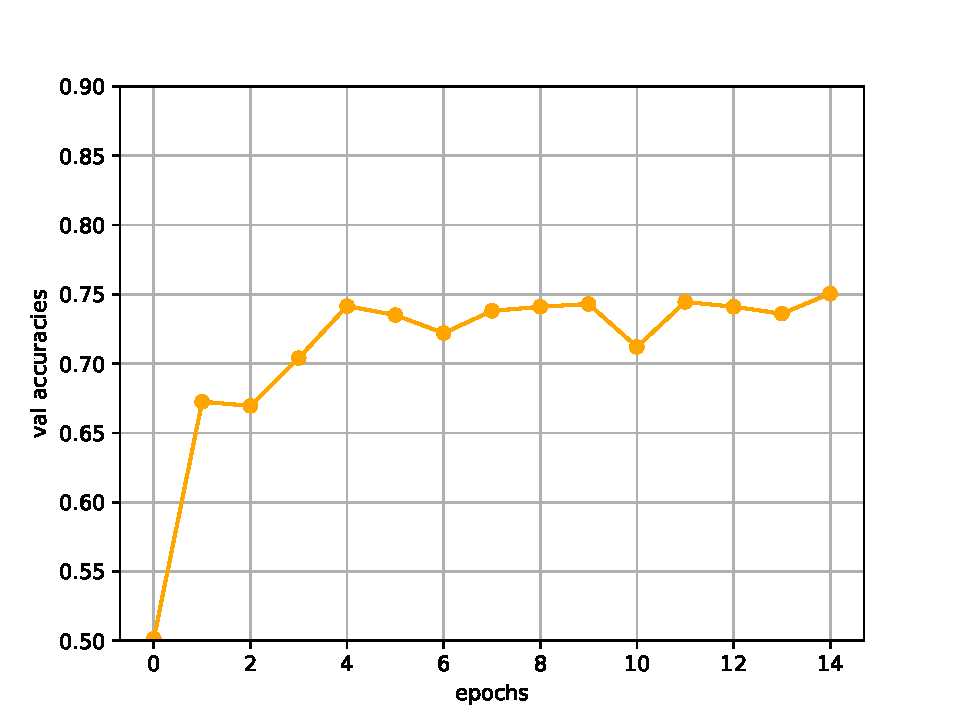
\includegraphics[width=\textwidth]{../figures/from_scratch_valaccs.pdf}
            \caption{Evolution of val accuracy of the from scratch model trained during 15 epoch.}
            \label{fig:image1}
        \end{subfigure}
        \hfill
        \begin{subfigure}[b]{0.45\textwidth}
            \centering
            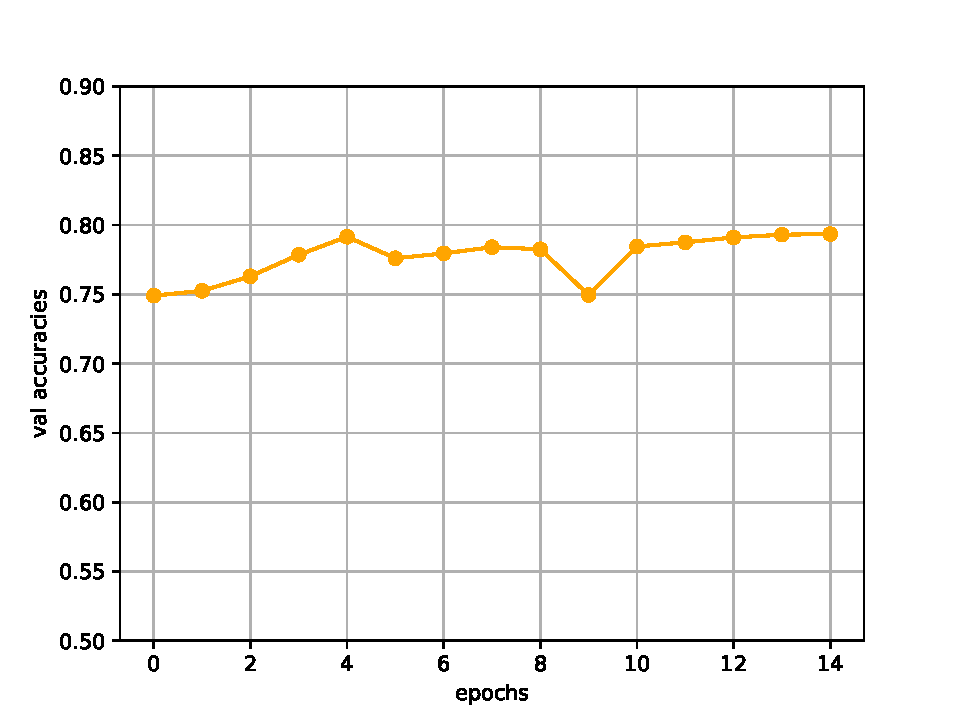
\includegraphics[width=\textwidth]{../figures/pretrained_valaccs.pdf}
            \caption{Evolution of val accuracy of the pretrained model trained during 15 epoch.}
            \label{fig:image2}
        \end{subfigure}
        \caption{Val accuracies observation of the 2 tested models.}
        \label{fig:figure}
    \end{figure}

    \subsection*{Interpretation of the results:} 
        The pretrained model generally performs better, with a higher peak accuracy $(0.81$ vs $0.76)$
        and average. The pretrained weights thus provide a better starting point, allowing the model
        to learn more effectively.
        \\
        As the learning rate is really small, those observations are quite normal, with
        a very low improvement of the val accuracy after 5-6 epochs.
        \\
        \\
        Additionnaly, the stabilization at 0.75 of the scratch model suggests that the model has
        difficulty to classify correctly. This could be due to insufficient training data
        (arround 1600 normal sentences), or maybe tuning better the hyperparameters that are
        tuned for fine-tuning and transfert learning. On the other hand,
        the pretrained model is better at distinguishing the two classes. However,
        this model has also variability in accuracy, and may need also more training data.
        \\
        For both models, the tendancy of constant evolution during epoch might be due
        to overfitting from training data.
        \\
        \\
        The pretrained model shows promise with higher peak accuracy, indicating that
        transfer learning is beneficial for your task. Further fine-tuning, data
        augmentation, and hyperparameter tuning can help improve both models' performance.

\section*{Question 5}
    Transformers used for language model pre-training are usually implemented with as a left-to-right
    architecture, which means that every tokens can only have informations from previous ones.
    In this notebook, we used the \texttt{TransformerEncoderLayer} from Pytorch, based on
    a traditional left-to-right approach. For language modeling tasks, it's well efficient.
    One problem is that is less adaptable when using those models for other specfic tasks. For instance,
    for what we do in this notebook, sentiment analysis, it could be more efficient to
    have access to all tokens of the sentences, as we want a general understanding of the
    text review and not just predict the futur word.\\
    \\
    One solution proposed in \cite{devlin2019bertpretrainingdeepbidirectional} is to use
    a bidirectional approach, such as Bidirectional RNNs/LSTMs (we can refer to the previous Lab session).
    Introduced in the BERT paper (\cite{devlin2019bertpretrainingdeepbidirectional}), they present
    masked language models, by masking tokens and predicting them based on the entire context
    (left and right) during the unsupervised task. This could lead to a better understanding of
    the global review. This kind of limitation task can be known as representation learning.
    \\
    With a unidirectional Language modelling, representation learning may be less robust
    for tasks that require understanding of the context (from both direction). In comparaison,
    Masked Language models can learn easily more contextually representations, as it must
    understand the entire sequence to predict the masked tokens.



%------------------------------------------------

\bibliographystyle{plain}
\bibliography{references} % citation records are in the references.bib document

\end{document}
